\documentclass[10pt]{article}

\usepackage[a4paper,margin=0.85in]{geometry}
\usepackage[T1]{fontenc}
\usepackage[utf8]{inputenc}
\usepackage{lmodern}
\usepackage[nopatch=footnote]{microtype}
\usepackage{amsmath,amssymb}
\usepackage{bm}
\usepackage{booktabs}
\usepackage{enumitem}
\usepackage{graphicx}
\usepackage{hyperref}
\usepackage{xurl}
\usepackage[numbers,sort&compress]{natbib}
\usepackage{tikz}
\usetikzlibrary{arrows.meta,positioning,shapes.geometric,fit,calc}

\title{LinStabPy: compressible stability and resolvent analysis}
\author{%
Gabriel Y.~R.~Hamada$^{1,2}$, Ricardo A.~S.~Frantz$^{3}$\\[0.75em]
\small $^{1}$ School of Mechanical Engineering, University of Campinas, Campinas, SP 13083-860, Brazil\\
\small $^{2}$ DynFluid, Arts et M\'etiers Paris / CNAM, 151 Bd de l'H\^opital, 75013 Paris, France\\
\small $^{3}$ Laboratory of Fluid Mechanics and Instabilities,\\
\small \'Ecole Polytechnique F\'ed\'erale de Lausanne, CH-1015 Lausanne, Switzerland%
}
\date{}

\begin{document}
\maketitle

\begin{abstract}
We present LinStabPy, an open Python framework for compressible linear
stability and resolvent analysis built around a shared discrete operator for
supplied base or mean flows. The discretization employs summation-by-parts finite differences on
curvilinear grids; the resulting sparse systems are solved through
PETSc/SLEPc.
A software layer reuses the same assembled operator across temporal stability,
spatial stability, and resolvent workflows. Independent operator checks,
fidelity assessment against the reference MATLAB implementation, and validation
in an oblique shock-wave/boundary-layer-interaction setting are collected in
the Supplementary Material. The implementation is released as the Python
package \texttt{linstabpy}.
\end{abstract}

\noindent\textbf{Keywords:} compressible stability; resolvent analysis;
linearized Navier--Stokes; sparse solvers; PETSc; SLEPc

\section{Introduction}

Linear stability and resolvent analyses remain standard tools for
compressible-flow problems once a reference state is already available from
simulation, experiment, or a separate base-flow solver
\citep{schmid2001stability,theofilis2011global,mckeon2010critical,towne2018spectral}.
In this setting the central object is the discrete linearized
operator, which---rather than the base-flow generator itself---supports
modal, nonmodal, and frequency-domain analyses.
The practical bottleneck is therefore twofold. One needs a trustworthy
compressible discretization, and one needs a solver stack that remains usable
when the resulting sparse systems become large.

LinStabPy builds on two public repositories: the
\texttt{LinStab2D} repository \citep{linstab2drepo,martini2024} and the
\texttt{resolvent4py} repository
\citep{resolvent4pyrepo,padovan2025resolvent4py,resolvent4pycgl}. The former provides the
compressible formulation on structured and curvilinear grids, including
summation-by-parts finite differences, boundary-condition recipes, and
resolvent analysis. The latter introduces reusable operator
abstractions for large-scale linear analyses. LinStabPy combines these layers:
a compressible discrete operator for supplied flows, an analysis interface
written in terms of that operator, and interchangeable PETSc/SLEPc solver
backends for direct and iterative linear-algebra workflows.

The surrounding software ecosystem is expanding. Packages such as
\texttt{BROADCAST} \citep{poulain2023broadcast},
\texttt{dNami} \citep{dnami2022}, and
\texttt{LightKrylov} \citep{kern2026lightkrylov} reflect growing open-source
activity around operator-based workflows and Krylov-based numerics; see
\citet{frantz2023krylov} for a review of Krylov methods in fluid-dynamics
applications.

LinStabPy addresses a narrower workflow than these broader packages.
Many users can obtain a nonlinear base or mean flow but lack a ready-to-use
compressible linear operator with the needed thermodynamic, curvilinear, and
boundary-condition support. LinStabPy fills that gap: the base or mean flow
is obtained from the user's own CFD or data-generation environment, and the
package discretizes the corresponding linearized operator for prototyping and
production-scale stability/resolvent calculations.

The main contribution is the framework itself: rather than reporting
new flow-physics findings, we provide a computational tool that turns
supplied compressible reference states into a discrete operator reusable
across temporal stability, spatial stability, and resolvent analyses.
The detailed formulation, verification protocol,
and benchmark results are collected in the Supplementary Material.

\section{Framework}

The framework takes as input a compressible base or mean flow together
with the mesh, finite-difference order, boundary-condition recipe, and filter
choices. Together, these define a fully discrete linearized operator.
Temporal stability, spatial stability, and resolvent analysis then act on that
shared operator or on derived shifted/block variants, while the sparse linear
algebra is handled through PETSc/SLEPc \citep{balay2025petsc,hernandez2005slepc}
with MUMPS direct factorization \citep{amestoy2001mumps} for eigenvalue
problems and either direct or iterative Krylov/preconditioning routes
\citep{saad2003iterative,benzi2002preconditioning} for resolvent analyses.

Because the operator is assembled explicitly as a sparse matrix, it pairs
naturally with direct sparse-LU factorization for the shift-invert inner
solves that eigenvalue problems require. This is distinct from the
time-stepper approach \citep{edwards1994krylov,barkley2008direct}, in which
the linearized operator is never formed and Krylov methods serve as the
\emph{outer} eigensolver acting on propagator snapshots; see
\citet{frantz2023krylov} for a review. The two approaches use ``Krylov
methods'' in different roles (outer iteration on the propagator versus inner
iteration on a shifted system), and the distinction matters for solver
selection: iterative inner solves encounter the non-normality of the shifted
operator directly, whereas the time-stepper outer loop avoids inversion
altogether. The Supplementary Material (Section~S6) discusses this point
in detail.

The framework separates physical assembly from operator analysis: changing the
finite-difference order, coordinate mapping, or boundary recipe affects only
the operator-construction step, not the downstream analysis logic. This design
builds on the compressible formulation of \citet{martini2024} while providing
a reusable software layer for current and future operator-based methods,
including the harmonic-resolvent extensions discussed in
\citet{padovan2020harmonic,padovan2022subharmonic,farghadan2025timestepping}.

\begin{figure}[t]
\centering
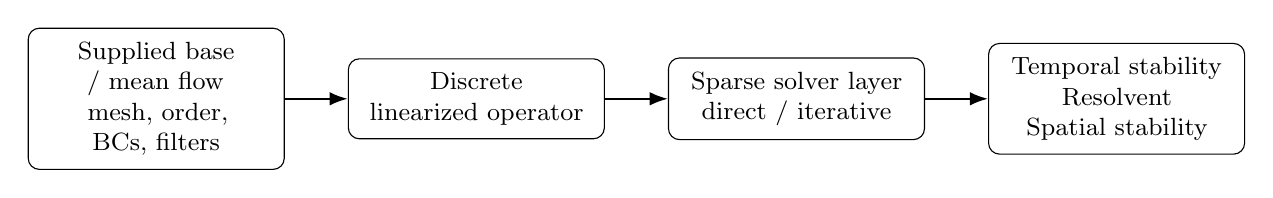
\begin{tikzpicture}[
  node distance=8mm,
  box/.style={draw, rounded corners, align=center, inner sep=5pt, font=\small, text width=2.9cm},
  arr/.style={-Latex, thick}
]
\node[box] (input) {Supplied base / mean flow\\mesh, order, BCs, filters};
\node[box, right=of input] (operator) {Discrete\\linearized operator};
\node[box, right=of operator] (solvers) {Sparse solver layer\\direct / iterative};
\node[box, right=of solvers] (analysis) {Temporal stability\\Resolvent\\Spatial stability};
\draw[arr] (input) -- (operator);
\draw[arr] (operator) -- (solvers);
\draw[arr] (solvers) -- (analysis);
\end{tikzpicture}
\caption{LinStabPy framework overview. User-supplied inputs define a discrete
linearized operator, which feeds stability and resolvent workflows through
a direct or iterative sparse solver layer.}
\label{fig:framework}
\end{figure}

\section{Verification and scope}

The Supplementary Material presents verification evidence in three parts:
two independent checks of the assembled discrete operator, fidelity assessment
through the five shipped Martini examples \citep{martini2024}, and validation
in the oblique SWBLI setting of Robinet \citep{robinet2007bifurcations} and
Song and Hao \citep{song2023global}. It also contains the compressible
linearized Navier--Stokes derivation, curvilinear and SBP discretization
details, solver configuration, the discrete Chu energy norm, and the
harmonic-resolvent extension.

\section{Code availability}

LinStabPy is available at \url{https://github.com/ricardofrantz/LinStabPy} as
the Python package \texttt{linstabpy}; release DOI and snapshot metadata will
be added in the final submission package.

\bibliographystyle{unsrtnat}
\bibliography{refs}

\end{document}
